\documentclass[../main.tex]{subfiles}
\begin{document}

% The question that arises immediately when considering ensemble learning is whether combining the outputs of members could possibly \textit{hurt} the generalisation error. If member models are random according to a random variable parameter $\Theta$, we can quantify this by comparing the ensemble loss to the loss of an expected member. This is exactly the ambiguity-effect (\ref{todo}).

% superfluous
% \marginnote{
%     \textit{Ambiguity-effect}, sometimes also called \textit{ensemble improvement} is defined as (see {thm:ambiguity-effect-decomp})
% $$
% \Mavg L(Y, q_{i}) - L(Y, \bar{q})
% $$
% for ensemble members $q_1, ..., q_M$, combiner $\bar{q}$ and loss function $L$.
% }

% We have yet to see if and when this quantity is non-negative. If so, combining individual models in an ensemble can not hurt performance. Further, we want to see how large this improvement actually is and whether on can construct better ensembles by adressing it explicitly.





\section{Diversity for the \zeroone-Loss}
\label{sec:diversity-zeroone}
While for Bregman divergences ensembling cannot hurt performance, this is not given for the general case. For the \zeroone-loss, a way forward is to impose assumptions on the performance of member models.
In the remainder of this section, we will review some assumptions that imply ensemble effectivity and show that they are in fact tightly related. We begin by focussing on binary classification problems and then briefly consider non-binary problems.


\begin{definition}
\label{def:zeroone-loss}
The \zeroone-loss between two outcomes is 
$$
\Lzo{Y}{Y'} \defeq \ind{Y \not= Y'}
$$
\end{definition}

The ensemble combiner implied by the \zeroone-loss is the plurality vote.
\marginnote{
    The proper term here would actually be \textit{plurality} vote since, for a class to win the vote, it is required to have more than $\nicefrac{1}{k}$ votes. Strictly speakin, a \textit{majority} vote win requires the majority of all votes, i.e. more than $\nicefrac{1}{2}$. For $k=2$, majority and plurality voting is equivalent.
    % TODO throughout what follows, try to resolve ambiguities between maj vote and plurality vote
}
\begin{definition} 
   \label{def:majority-vote} 
    (Majority/Plurality vote combiner) For a $k$-class classification problem, the majority vote combiner is defined as
$$
\bar{q}(X) = \arg\min_{z \in [k]} \mathbb{E}_{\Theta}\left[ \Lzo{z}{q_{\Theta}} \right]  
$$
\end{definition}
This assumes that each member model predicts a single class, although this does not imply that member models must necessarily be trained based on the \zeroone-loss, too. If a member predicts a class, we also say that the member \textit{votes} for that class.

In the remainder of this section, we will analyse classification ensembles as measured by the \zeroone-loss. 
% TODO give an overview what where going to talk about
A basic quantity for this will be the ratio of members that are incorrect for a given example-outcome pair.

\begin{definition}
For a distribution of members constructed according to input data $D = (D_{1}, \dots, D_{M})$ and parameters $\Theta = (\Theta_{1}, \dots, \Theta_{M})$, the ratio of incorrect ("wrong") members is
$$
W(X,Y) \defeq \mathbb{E}_{D, \Theta}\left[ \Lzo{Y}{q_{D, \Theta}(X)} \right] \approx \Mavg \Lzo{Y}{q_{i}(X)}
$$
As with other variables, we sometimes omit explicitly stating the dependence on $(X,Y)$. Further, we write $W_{\Theta} \defeq \mathbb{E}_{\Theta}\left[ \Lzo{Y}{q_{D, \Theta}} \right]$. For the complement, we write $\compl{W} \defeq 1 - W$
\end{definition}

\begin{lemma} (\cite{theisen_WhenAreEnsembles_2023}) The ratio of incorrect members in expectation over all examples is equal to the error rate of an average member.
    \begin{align*} 
    \mathbb{E}_{(X,Y) }\left[ W  \right]  = \mathbb{E}_{(X,Y) }\left[ \mathbb{E}_{D,\Theta}\left[ \Lzo{Y}{q_{D,\Theta}(X)} \right]  \right]  = \mathbb{E}_{D,\Theta}\left[ \mathbb{E}_{(X,Y) }\left[ \Lzo{Y}{q_{D,\Theta}(X)} \right]  \right] 
    \end{align*}
    \label{thm:W-lzo}
\end{lemma}


% TODO emphasize that this is sort of a "classic" bound and we provide it for context
\paragraph{A simple bound} Using Markov's inequality, we can readily upper-bound the error of the ensemble in terms of expected errors of the members~\cite{theisen_WhenAreEnsembles_2023}
\sidenote{ Markov's inequality states that for a nonnegative random variable $X$ and $a > 0$ $$ \mathbb{P}\left[X \geq a\right] \leq \frac{\mathbb{E}\left[X\right]}{a}.$$ 
% The final equality is due to that one can swap the order of expectations in $\mathbb{E}_{D}\left[ W_{\Theta} \right] = \mathbb{E}_{{D}}\left[ \mathbb{E}_{\Theta}\left[ \ind{q_{\Theta}(X) \not= Y} \right] \right] = \mathbb{E}_{\Theta}\left[  L(q_{\Theta}) \right]$. 
}
.
% TODO notation
$$
0 \leq \mathbb{E}_{}\left[ \Lzo{Y}{\bar{q}} \right] = \prob{}{W \geq \kappa} \leq \prob{}{W \geq \nicefrac{1}{2}} \leq 2 \mathbb{E}_{}\left[ W \right] 
$$
% TODO actually provide example 1 from theisen paper, that's easy to understand and gives intuition
While there exist examples for which this upper bound is tight \cite{theisen_WhenAreEnsembles_2023}, it is reasonable to suspect that the ensemble being worse by a factor of two is only a pathological case and not relevant for practise.

% Recall that, due to the ambiguity-effect decomposition (see \ref{thm:ambig-effect-decomp}), ensembling can not hurt performance if and only if diversity-effect is non-negative. Figure \ref{fig:pathological-example} gives an example of an ensemble with negative diversity-effect. Although such cases can be expected to rarely appear in practise, the question still stands what characteristics make a majority vote ensemble work. 

\subsection{Diversity in binary classification problems}

We begin by considering binary classification problems which have $k=2$ two possible outcomes. 
The special property of binary classification problems is that any vote which is not correct is automatically a vote for the single other class. In other words, diversity can be measured in terms of disagreement between members. 
This is not given for problems with $k>2$ where an incorrect vote might correspond to any other class. We will see that, in this case, diversity will be measured in terms of differences in \textit{correctness} of members.

% While diversity-effect (in expectation over $(X,Y)$) is non-negative for ensembles of weak-learners (see theorem \ref{thm:todo}), there may still be example-outcome pairs that contribute negatively to the expectation, as illustrated in figures \ref{fig:zeroone-div-eff-good} and \ref{fig:zeroone-div-eff-bad}

\begin{marginfigure}
    \label{fig:zeroone-div-eff-good}
    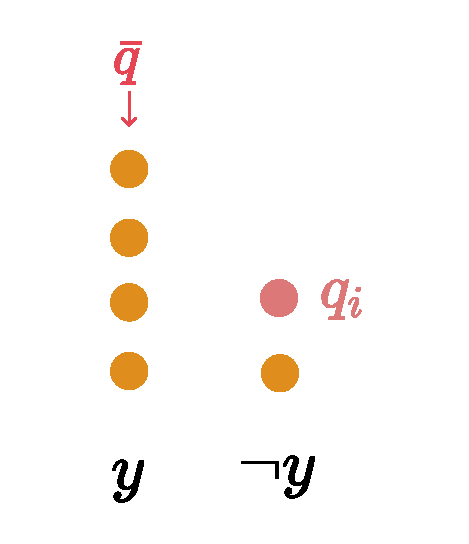
\includegraphics[width=0.8\textwidth]{figma-illustrations/zeroone-div-effect-good.pdf}
    \caption{
        Example of the effect of a member's vote $q_i$ on the diversity on a point for which the ensemble majority vote is correct.
    Example where $q_i$ has positive contribution to the diversity effect term, i.e. 
$\Lzo{y}{q_{i}} - \Lzo{y}{\bar{q}} = 1$. The member $q_{i}$ is incorrect but due to the discreteness of the majority vote combiner, the ensemble performance does not suffer -- unless the majority vote is tipped. Any correct vote while the ensemble already is correct is effectively "wasted" and incorrect votes correspond to diversity.
}
\end{marginfigure}
\begin{marginfigure}
    \label{fig:zeroone-div-eff-bad}
    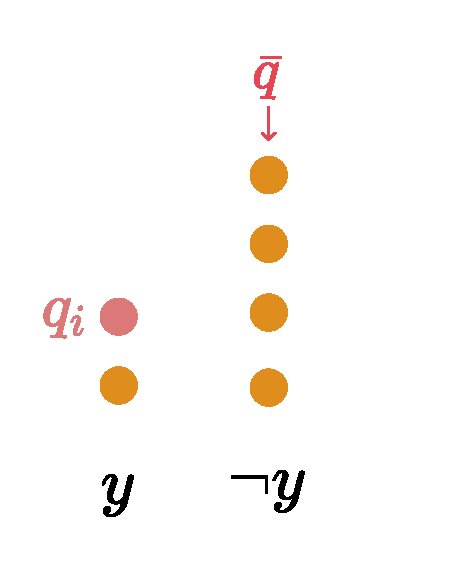
\includegraphics[width=0.8\textwidth]{figma-illustrations/zeroone-div-effect-bad.pdf}
    \caption{
    Example where $q_i$ has negative contribution to the diversity effect term, i.e. 
$\Lzo{y}{q_{i}} - \Lzo{y}{\bar{q}} = -1$. Any further incorrect vote while the ensemble is already incorrect would be wasted. The negative effect here eventually results in the \zeroone-loss of $1$.
}
\end{marginfigure}

% TODO establishing link to theisen theory also connects all of that stuff specific to the 0/1-loss to ambig theory, which is general

% TODO these definitions should come before the theisen theory
% TODO this is only for binary classification or what? has been generalised?
The dichotomy of binary classification problems allows us to succinctly express the diversity-effect.
\begin{lemma} (\cite{brown_GoodBadDiversity_2010})
For a classification problem with $k=2$ classes, let $y, \bar{q} \in \{ -1, 1 \}$. It then holds that
$$
\Mavg \left[\Lzo{y}{q_{i}} - \Lzo{y}{\bar{q}}\right] 
= (y \cdot \bar{q}) \Mavg \Lzo{\bar{q}}{q_{i}} \in \{-1, 0, 1\}
$$
\end{lemma}
\begin{proof} Let $y, \bar{q} \in \{ -1, 1 \}$.
\begin{itemize}
\item Assume the ensemble is correct, i.e. $y=\bar{q}$. Then $\Lzo{y}{\bar{q}} = 0$ and the left-hand-side equals $\Mavg\Lzo{y}{q_{i}} = \Mavg\Lzo{\bar{q}}{q_{i}}$. Further, $y \cdot \bar{q} = 1$.
\item Assume the ensemble is incorrect, i.e. $y \not= \bar{q}$. Then $y \cdot \bar{q} = -1$ and, for the left-hand-side, we can write
$$
\Mavg \left[\Lzo{y}{q_{i}}\right] - 1 = - \left(1 - \Mavg \Lzo{y}{q_{i}}\right) = - \left(\Mavg \Lzo{\bar{q}}{q_{i}} \right)
$$
using that, since $y \not= \bar{q}$, $\left(  1 - \Mavg \Lzo{y}{q_{i}}\right) = \Mavg \Lzo{\bar{q}}{q_{i}}$.
\end{itemize}
\end{proof}
% TODO rather, the below should be in a theorem box and the above should be the motivation/derivation/proof
% This shows that, for binary classification under \zeroone-loss, diversity-effect can be decomposed exactly between points that contribute positively or negatively to the overall loss.
%  Starting from the 
% ambiguity-effect decomposition \ref{sec:ambiguity-effect-decomp}:
\marginnote{
An intuition of this is also that of "wasted votes": Under the majority vote combiner, for the ensemble to be correct, we require only at least half of the members to be correct. Any higher ratio of correct ensemble members does not improve the ensemble performance on this point and these can be seen as "wasted". Likewise, the ensemble is incorrect if not more than half of the members are correct. Any positive votes do not influence the ensemble improvement and can be considered "wasted". 
}

We can divide the range of $X$ into two disjoint subsets. Let $X_{+}$ be the examples on which the ensemble is correct. Ambiguity on these points has a decreasing effect on the overall ensemble error. Let $X_{-}$ be the examples on which the ensemble is incorrect. Ambiguity on these points has an increasing effect on the overall ensemble error. This yields a decomposition into \textit{good} and \textit{bad} diversity.

% TODO instead give this in terms ambiguity decomp here
\begin{corollary} (\cite{brown_GoodBadDiversity_2010})
    \label{thm:good-bad-diversity}
For a classification problem with $k=2$ classes, let $y, \bar{q} \in \{ -1, 1 \}$. It then holds that
\begin{align*}
\mathbb{E}_{X}\left[   L(Y, \bar{q}) \right] 
&= 
% \mathbb{E}_{X}\left[    \Mavg \Lzo{Y}{q_{i}}  \right]
% -
% \mathbb{E}_{X}\left[   \Mavg L(Y, q_{i}) - L(Y, \bar{q}) \right] \\
% &= 
% \mathbb{E}_{X}\left[ \Mavg \Lzo{Y}{q_{i}} \right] - \mathbb{E}_{X}\left[ (y \cdot \bar{q}) \Mavg \Lzo{\bar{q}}{q_{i}} \right]  \\
% &= 
\mathbb{E}_{X}\left[    \Mavg \Lzo{Y}{q_{i}}  \right] \\
&- 
\underbrace{
\mathbb{E}_{X_{+}}\left[ \Mavg \Lzo{\bar{q}}{q_{i}} \right]  
}_{\text{"good" diversity}} \\
&+ 
\underbrace{
\mathbb{E}_{X_{-}}\left[ \Mavg \Lzo{\bar{q}}{q_{i}} \right] 
}_{\text{"bad" diversity}}
\end{align*}
\end{corollary}
% TODO how does this relate to competence / weak learner assumption?

% TODO make indices, notation consistent and more comparable with other theorems
% TODO give a bit of reasoning why formally we can decompose expectation into X+, X-
% TODO key difference to covariance arguments is that members only need to be different to the combiner, and not necessarily disagree *with each other*?
% TODO marginfig with these functions
% TODO also intuition how other ensemble members "pulls" combiner into other direction
% TODO ok well obviously noted by kuncheva, but not exploited
%  Starting from the ambiguity decomposition:
% $$
% \Lzo{y}{\bar{q}} 
% = \Mavg \Lzo{y}{q_{i}} - \left(\Mavg   \Lzo{y}{q_{i}} - \Lzo{y}{\bar{q}} \right)
% $$
% If $x \in X_{+}$, i.e. $\bar{q}(x) = y$:
% $$
% \Lzo{y}{\bar{q}} = 
% \Mavg \Lzo{y}{q_{i}} - \left(\Mavg   \Lzo{y}{q_{i}} - 0 \right) = 0
% $$
% If $x \in X_{-}$, i.e. $\bar{q}(x) \not= y$:
% $$
% \Lzo{y}{\bar{q}} = 
% \Mavg \Lzo{y}{q_{i}} - \left(\Mavg   \Lzo{y}{q_{i}} - 1 \right) = 1
% $$       

Note that this is a special case of the ambiguity-effect decomposition of \cref{thm:ambig-effect-decomp}.
There is a tradeoff between average member error and diversity. Here, however, diversity is not always beneficial. On points where the ensemble is incorrect, disagreements have a negative effect on the overall ensemble error.
In other words, for majority vote ensembles, diversity is only beneficial \textit{on points at which the ensemble can actually afford to be diverse}. 

Further, from corollary \ref{thm:good-bad-diversity}, one can already see that the ensemble improvement (i.e. diversity-effect) in binary classification problems is only non-negative if good diversity outweights bad diversity.

% As can be seen from the ambiguity decomposition of theorem \ref{thm:ambig-effect-decomp}, for diversity to be beneficial it has to mitigate the average member error. 
% % TODO clarify above sentence
% However, to the best of our knowledge, it has not yet been exploited that diversity is measured \textit{per point}.
% % TODO cite that paper in margin that does this via human-in-the-loop

Good and bad diversity can be expressed solely in terms of the ratio of incorrect members. 
\begin{lemma} 
    \label{thm:good-bad-diversity-W}
    $\star$ Let $y$ be the true outcome for a given example. Let $\neg y$ be an outcome that is not $y$. Write $\Lzo{q_i}{\neg y} \defeq \sum_{k \not= y} \Lzo{q_i}{k}$ for the indication whether $q_i$ is incorrect. Then the following identities hold.
% TODO y always first in losses
\begin{align*}
\mathbb{E}_{X_{+}}\left[ \Mavg \Lzo{q_{i}}{\bar{q}} \right] &=
\mathbb{E}_{X_{+}}\left[ \Wmem \right]   \\
\mathbb{E}_{X_{-}}\left[ \Mavg \Lzo{q_{i}}{\bar{q}} \right]  &= \mathbb{E}_{X_{-}}\left[ \Mavg  \Lzo{q_{i}}{\neg y} \right]  \\
&=
\mathbb{E}_{X_{-}}\left[ 1 - \Wmem \right]
\end{align*}
Analogous equalities hold in expectation over member parameter $\Theta$.
\end{lemma}

\subsection{Ensembles of weak Learners}

The following result holds for an arbitrary number of classes. Note that this is also the assumption enabling \cref{thm:breiman}.

\begin{definition} 
    % TODO relate to margin defs
    % TODO cite
   \label{def:weak-learner}  (Weak learner, \cite{theisen_WhenAreEnsembles_2023,wood_BiasVarianceDecompositionsMargin_2022})
   A model $q_{\Theta}$ is a weak learner if and only if performs better than randomly guessing.
$$
\mathbb{E}_{(X,Y) }\left[ \Lzo{Y}{q_{\Theta}} \right] \geq \nicefrac{1}{2}
$$
\end{definition}

\begin{theorem} 
    \label{thm:weak-learner-ensembles-nonnegative}
    (\cite{wood_UnifiedTheoryDiversity_2023}) In an ensemble of weak learners, diversity-effect is non-negative:
$$
% TODO notation
\mathbb{E}_{D}\left[ 
\mathbb{E}_{Y}\left[ 
\Mavg \Lzo{Y}{q_{i}} - \Lzo{Y}{\bar{q}}
\right] 
\right] 
~ ~ \geq ~ ~ 0
$$
\end{theorem}

A proof is given in \cite{wood_UnifiedTheoryDiversity_2023}. For binary classification problems, one can see that the weak learner condition implies that good diversity outweighs bad diversity.

\subsection{Competence in binary classification problems}

% TODO relate to weak learner condition, wood23 thm14
\citeauthor{theisen_WhenAreEnsembles_2023} consider the question of ensemble improvement under the \zeroone-loss. They define an assumption on the ratio of inccorect members.

\begin{marginfigure}
    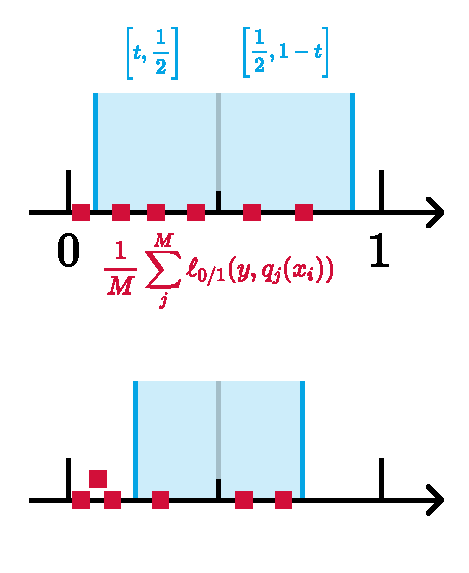
\includegraphics[width=\textwidth]{figma-illustrations/competence.pdf}
    \caption{
        Illustration for the competence condition \ref{def:2-competence} for binary classification. \tcircle{orange} Squares correspond to pairs $(X,Y)$ from the joint distribution of examples and outcomes. For each of these pairs, the average/expected member error $W_{\Theta}(X,Y) \approx \Mavg \Lzo(y, q_i)$ is the ratio of incorrect members. The center $\nicefrac{1}{2}$ is the majority vote threshold. Informally, an ensemble is competent, if, for any two \tcircle{ctpblue} intervals defined by $t$ left and right of the threshold, more examples are in the left part. For the upper example, this holds. For the lower example, even though many examples are classified correctly by many members, the ensemble is \textit{not} competent.
        % TODO come back to this from persective of good/bad div
        % TODO emphasize that this is motivation for *dis*couraging disagreement on incorrect points (bad div)
    }
    \label{fig:competence}
\end{marginfigure}
% TODO k-competence also shows rigorously how with larger k, there is less room for diversity
% TODO considerations of k-competence (namaly the thresholds) having an influence on weighting? I think so
% TODO this might also be a motivation for DRF approach
 % TODO emphasize this insight

\begin{definition} 
   \label{def:2-competence} 
    ($2$-competence, \cite{theisen_WhenAreEnsembles_2023}) An ensemble is $2$-competent iff
$$
\forall t \in \left[ 0, \nicefrac{1}{2} \right]: ~ \prob{(X,Y) }{W(X,Y)  \in \left[ t, \nicefrac{1}{2} \right]} ~ ~  \geq ~ ~ \prob{(X,Y) }{W(X,Y) \in \left[ \nicefrac{1}{2}, 1-t \right]}
$$
\end{definition}
The condition is illustrated in \cref{fig:competence}.  
% TODO re-integrate
% The weak learner assumption is a special case of this for $t = 0$.  % TODO Check
% Ensembles of weak learners are competent and as such, this alternatively indirectly proves theorem \ref{thm:weak-learner-ensembles-nonnegative}.
% TODO elaborate, maybe star

\begin{proposition} $\star$
\label{thm:weak-learner-competence}
The weak learner condition of \cref{def:weak-learner} is a special case of $2$-competence.
\end{proposition}
\begin{proof}
The weak learner condition implies that, also in expectation
$$
\mathbb{E}_{\Theta,D}\left[ \mathbb{E}_{(X,Y) }\left[ \Lzo{Y}{\bar{q}} \right]  \right]  \geq \nicefrac{1}{2}
$$
Consequently, using \cref{thm:W-lzo}, we have
\begin{align*}
\nicefrac{1}{2} &\leq \mathbb{E}_{\Theta,D, (X,Y) }\left[ \Lzo{Y}{\bar{q}} \right]  = \mathbb{E}_{(X,Y) }\left[ W \right]  \\
& ~\leftrightarrow~ \mathbb{E}_{(X,Y) }\left[ ~\ind{W \in \left[ 0, \nicefrac{1}{2} \right]}  \right] = \prob{(X,Y) }{W \in [0, \nicefrac{1}{2}]} = 1
\end{align*}
\end{proof}

The $2$-competence condition was used to show two kinds of results \cite{theisen_WhenAreEnsembles_2023}:
\begin{itemize}
	\item In $2$-competent ensembles, diversity-effect is non-negative.
	\item For $2$-competent ensembles, the ensemble generalisation error is bounded from above and below by linear functions of the expected disagreement between two members.
\end{itemize}

One can see that competence is essentially determined by the distribution of examples $(X,Y)$ over the range of $W(X,Y)$ which is divided by the majority vote threshold $\nicefrac{1}{2}$. We have already seen that, similarly, diversity-effect in its apparent form of good and bad diversity is determined by just the same characteristics. How are these two related?
We will argue that non-negative diversity-effect is in fact equivalent to a notion of competence generalised to $k > 2$ classes. Unless otherwise noted, all expectations and probabilites are over the distribution of $(X,Y)$.

While proving that $2$-competence implies non-negative diversity-effect, \citeauthor{theisen_WhenAreEnsembles_2023} establish the following fact.
\begin{align}
\label{eq:competence-lemma2}
\text{ens. $2$-competent} ~\leftrightarrow~ \mathbb{E}_{}\left[ W~\ind{W < \nicefrac{1}{2}} \right] \geq \mathbb{E}_{}\left[ 
\compl{W}~\ind{\compl{W} \leq \nicefrac{1}{2} } 
\right] 
\end{align}
We can rearrange this into a more suggestive form. Recall that $W = \mathbb{E}_{D, \Theta}\left[ \Lzo{Y}{q_{D,\Theta}(X)} \right]$. We now split off the expectation over $D$ and instead consider $W_{\Theta} = \mathbb{E}_{\Theta}\left[ \Lzo{Y}{q_{D, \Theta}(X)} \right]$. Rearranging the above and exploiting the linearity of expectation, we obtain
$$
d \defeq \mathbb{E}_{(X,Y),D }\left[ W_{\Theta} ~\ind{W_{\Theta} < \nicefrac{1}{2}} \right]  - \mathbb{E}_{(X,Y) ,D}\left[ \compl{W_{\Theta}} ~\ind{\compl{W_{\Theta}} \leq \nicefrac{1}{2} } \right] ~ ~ \geq ~ ~  0
$$
The indicator functions are mutually exclusive and can thus be understood as a case distinction. With slight abuse of notation, where the expectations are only over the subset of the distribution for which the case condition holds, we can write
$$
d = 
\begin{cases}
\mathbb{E}_{}\left[ W_{\Theta} \right] & \leftrightarrow W_{\Theta} < \nicefrac{1}{2} \\[1em]
\mathbb{E}_{}\left[ \compl{W_{\Theta}}  \right]  = \mathbb{E}_{}\left[ 1 - W_{\Theta} \right]  & \leftrightarrow \compl{W_{\Theta}} \leq \nicefrac{1}{2} 
\end{cases}
$$

For $k=2$, the majority vote threshold is $\nicefrac{1}{2}$ and thus the conditions correspond exactly to the ensemble being either correct or incorrect.

\begin{align}
\label{eq:gen-error-ratio-binary}
k = 2 ~\rightarrow~ 
\begin{cases}
W_{\Theta}  < \nicefrac{1}{2} ~\leftrightarrow~  \bar{q}(X) = Y \\[1em]
\compl{W_\Theta }  \leq \nicefrac{1}{2} ~\leftrightarrow~ \bar{q}(X) \not= Y
\end{cases}
\end{align}

% For $k=2$, the cases of \ref{just-above} correspond directly to the cases of the ensemble being correct or incorrect of equation \ref{eq:binary-classification-cases}. 
Recalling the characterisation of good and bad diversity of lemma \ref{thm:good-bad-diversity-W}, we can see that $d$ is nothing else but the diversity-effect. This means that non-negative effect is exactly equivalent to $2$-competence for a classification problem with $k=2$ classes.
% TODO if we want to make this more formal, we can use the arguments of theisen, proving thm 1 from lemma 2
Moreover, it is important to note that the gap of equation \ref{eq:competence-lemma2} and consequently the gap in the definition of $2$-competence (\cf \ref{def:2-competence}) is exactly the diversity-effect and exactly measures the ensemble improvement. In other words, we can now speak about the degree of competence of an ensemble.

\subsection{Competence and Diversity in non-binary classification problems}
\label{sec:k-competence}
% TODO maybe repeat what is ref'd here in margins
% Due to \ref{eq:gen-error-ratio-binary}, we can now see that for $k=2$, the other direction also holds: Any ensemble with non-negative diversity-effect also is competent. 
For $k>2$, the equivalence between the correctness of the ensemble and less than half of the members being incorrect (\cf \ref{eq:gen-error-ratio-binary}) is not given. While it is sufficient (a class with more than $\nicefrac{1}{2}M$ votes will win any plurality vote), it is not necessary: a plurality vote can be won with less than $\nicefrac{1}{2}M$ votes. Thus, there are ensembles which have non-negative diversity-effect (ensemble improvement) that are not $2$-competent. % TODO areas of wood23 fig20

The key difference is that for $k>2$, the voting threshold for a pair $(X,Y)$ is no longer the same value for all examples. Since a class wins if and only if it has more votes than any other class, the voting threshold depends on the distribution of class votes, which is potentially different for any pair $(X,Y)$. Nevertheless, there is still \textit{a} classification threshold, namely the ratio of votes for the next-best class. Because we will be considering the ratio of incorrect votes as a basic quantity, we will now define it from the reciprocal perspective:
$$
\kappa (X,Y) = 1 - \max_{Z \not= Y} \mathbb{E}_{\Theta}\left[ ~\ind{q_{\Theta} = Z} \right] 
$$
and it holds that
\marginnote{
    Let $$t \defeq \max_{Z\not=Y} \mathbb{E}_{\Theta}\left[ ~\ind{q_{\Theta} = Z} \right]$$ Then
    \begin{align*}
    \bar{q} = y & ~\leftrightarrow~ \compl{W}  \geq t \\
    & ~\leftrightarrow~ W = 1 - \compl{W}  < 1 - t = \kappa \\
    \end{align*}
    and
    \begin{align*}
    \bar{q} \not= y & ~\leftrightarrow~ \compl{W}  < t \\
    & ~\leftrightarrow~ 1 - \compl{W}  \geq 1-t = \kappa \\
    & ~\leftrightarrow~ 1 - (1 - \compl{W} )\leq 1-\kappa \\
    & ~\leftrightarrow~ \compl{W}  \leq 1 - \kappa
    \end{align*}
}
$$
\begin{align}
W_{\Theta} <& \kappa  & ~\leftrightarrow~ \bar{q}(X) = Y \\ 
\compl{W_{\Theta}} \leq& 1-\kappa  & ~\leftrightarrow~ \bar{q}(X) \not= Y
\end{align}
$$

% TODO use sth else than kappa or tildek, this is confusing
% TODO give some nicer intuition about how I came up with this idea in the first place : something like "ah if we just had that other threhsold here, all would bef ine"
% TODO check whether these are still correct
% \begin{marginfigure}
%     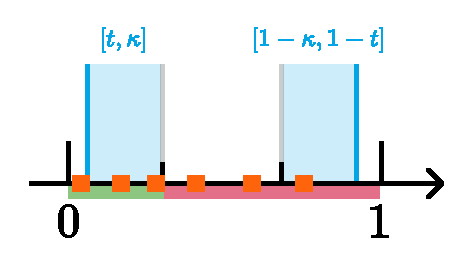
\includegraphics[width=\textwidth]{figma-illustrations/k-competence.pdf}
%     \label{fig:k-competence}
%     \caption{
%         Illustration for the $k$-competence condition \ref{def:k-competence}. 
%         % TODO right half is interesting... right half is exactly bad diversity, right?
%         % TODO implies that the kink in the weighting fn should be at kappa
%         % does this explain why it works so much better for spambase-openml, which has 2 classes, and not so well for other datasets?
%     }
% \end{marginfigure}
% \begin{marginfigure}
%     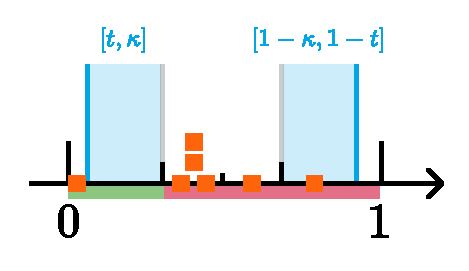
\includegraphics[width=\textwidth]{figma-illustrations/k-competence-counterexample.pdf}
%     \label{fig:k-competence-counterexample}
%     \caption{
%         The above ensemble is $2$-competent, but not $3$-competent.
%         $k$-competencies are not comparable as they are measures for completely different learning tasks.
%     }
% \end{marginfigure}
\begin{definition} $\star$ ($k$-competence)
   \label{def:k-competence} 
    An ensemble is $k$-competent iff
$$
\forall t \in [0,1]:
\prob{(X,Y) }{W \in \left[ t, \kappa \right]}
\geq \prob{(X,Y) }{W \in \left[ 1-\kappa, 1-t \right]}
$$
for $ \kappa \defeq 1 - \max_{Z \not= Y} \mathbb{E}_{\Theta}\left[ ~\ind{q_{\Theta} = Z} \right]$.
\end{definition}

% TODO relate to 2-competence
% TODO not correct
% For classification problems with $k=2$, $k$-competence is exactly $2$-competence as of definition \ref{def:2-competence} since the voting threshold is always $\nicefrac{1}{2}$.

\citeauthor{theisen_WhenAreEnsembles_2023} showed that $2$-competence implies non-negative diversity-effect. 
We now show that a very similar line of argument using $k$-competence actually holds in both directions.

\begin{theorem} $\star$ Consider an ensemble for a $k$-class classification problem. Then
$$
\text{$k$-competence}  ~ ~ ~\leftrightarrow~ ~ ~  \text{diversity-effect} \geq 0
$$
\label{thm:k-competence-diversity-effect}
\end{theorem}

The main work lies in establishing the following lemma, which is a generalised form of equation \ref{eq:competence-lemma2}. 

\begin{lemma} $\star$ (Generalised from \cite{theisen_WhenAreEnsembles_2023}) \label{thm:lemma-2} For an increasing function $f$ with $f(0)=0$, it holds that
$$
\text{$k$-competence}  ~\leftrightarrow~ \mathbb{E}_{}\left[ f(W) ~\ind{W < \kappa} \right] \geq \mathbb{E}_{}\left[ f(\compl{W}) ~\ind{\compl{W} \leq \kappa } \right]  
$$
where $ \kappa \defeq 1 - \max_{Z \not= Y} \mathbb{E}_{\Theta}\left[ ~\ind{q_{\Theta} = Z} \right]$.
\end{lemma}
\begin{proof}

We begin by observing that, for all $x \in [0,1]$
\marginnote{
\begin{align*}
& \prob{}{W \in [1-\kappa,1-x]} ~\ind{x \leq \kappa} \\
=& \prob{}{W \in [1-\kappa,1-x ]} ~\ind{ 1-x > 1-\kappa } \\
=& \prob{}{W ~\ind{W > 1-\kappa} ~ < ~ 1-x} \\
=& \prob{}{W ~\ind{\compl{W} \leq \kappa } ~ < ~ 1-x} \\
=& \prob{}{\compl{W} ~\ind{\compl{W} \leq \kappa } ~ \geq ~ x }
\end{align*}
}
\begin{align*}
\prob{}{W \in [x, \kappa] } \cdot ~\ind{x \leq \kappa } &= \prob{}{W ~\ind{W < \kappa} ~ \geq ~ x} \\
\prob{}{W \in [1-\kappa,1-x]} \cdot ~\ind{x \leq \kappa} &= \prob{}{\compl{W} ~\ind{\compl{W} \leq \kappa } ~ \geq ~ x }
\end{align*}
where the first factors on the left-hand-side appear in the definition of $k$-competence.
Since $W$ is nonnegative, using that $\mathbb{E}_{}\left[ X \right] = \int \prob{}{X \geq x} \, dx$, we can conclude that, for any $x \in [0,1]$
\begin{align*}
\text{($k$-comp.)}  &~\leftrightarrow~  
\prob{}{W ~\ind{W < \kappa} ~ \geq x} 
~ ~ \geq ~ ~
\prob{}{\compl{W} ~\ind{\compl{W} \leq \kappa } ~ \geq x } \\
% & ~\leftrightarrow~
% \prob{}{f(W) ~\ind{W < \kappa} ~ \geq x} 
% ~ ~ \geq ~ ~
% \prob{}{f(\compl{W}) ~\ind{\compl{W} \leq \kappa } ~ \geq x } \\
& ~\leftrightarrow~
\mathbb{E}_{}\left[ W ~\ind{W < \kappa} \right] ~ ~ \geq ~ ~ \mathbb{E}_{}\left[ \compl{W} ~\ind{\compl{W} \leq \kappa }  \right] 
\end{align*}
\end{proof}
Using this, we can now directly prove theorem \ref{thm:k-competence-diversity-effect}.

\begin{proof} (For \cref{thm:k-competence-diversity-effect}, generalised from \cite{theisen_WhenAreEnsembles_2023})
    \begin{align*}
        0 &= \mathbb{E}_{}\left[ (W-1)~\ind{W \geq \kappa} \right]  - \mathbb{E}_{}\left[ (W-1) ~\ind{W \geq \kappa} \right]  \\
        &= \mathbb{E}_{}\left[ (W-1)~\ind{W \geq \kappa} \right]  + \mathbb{E}_{}\left[ (1-W)~\ind{W \geq \kappa} \right]  \\
        &= \mathbb{E}_{}\left[ (W-1)~\ind{W \geq \kappa} \right]  + \mathbb{E}_{}\left[  \compl{W} ~\ind{\compl{W} < \kappa} \right]   \\
    \end{align*}
    Applying lemma \ref{thm:lemma-2} for $f = \text{id}$ to the second term yields
    % TODO need to make clearer that not only inequality holds but the gap actually *is* diversity-effect
    \begin{align*}
        & \mathbb{E}_{}\left[ (W-1)~\ind{W \geq \kappa} \right]  + \mathbb{E}_{}\left[  \compl{W} ~\ind{\compl{W} < \kappa} \right]   \\  
        \leq~ &  \mathbb{E}_{}\left[ (W-1)~\ind{W \geq \kappa} \right]  + \mathbb{E}_{}\left[ W ~\ind{W < \kappa} \right] 
    \end{align*}
    The above already is nothing but the diversity-effect:
    \begin{align*}
        0 \leq& \mathbb{E}_{}\left[ (W-1)~\ind{W \geq \kappa} \right]  + \mathbb{E}_{}\left[ W ~\ind{W < \kappa} \right]  \\
        = & \mathbb{E}_{}\left[ W  \right]  - \mathbb{E}_{}\left[ ~\ind{W \geq \kappa} \right]  \\
        = & \mathbb{E}_{}\left[ W \right]  - \prob{}{W \geq \kappa}
    \end{align*}
    The first term is the ratio of incorrect members in expectation over all examples and is equal to the error rate of an average member (see \cref{thm:W-lzo})
    The second term is the ensemble error. 
\end{proof}

\subsection{Bounds for competent ensembles}

$2$-competence was used to show upper and lower bounds for the diversity-effect \cite{theisen_WhenAreEnsembles_2023}. Now we show that, with minor adjustments, the same bounds can be derived from $k$-competence. 
Besides giving performance guarantees, these bounds are interesting due to that they are expressed in terms of disagreements between members -- which until now we have only seen for Bregman divergences.

\begin{theorem} 
\label{thm:theisen-upper}
    (Upper bound) In $k$-competent ensembles,
$$
\mathbb{E}_{}\left[ W \right] - \prob{}{W \geq \kappa} \leq \mathbb{E}_{\rho, \rho'}\left[ D(q_{\rho}, q_{\rho'}) \right]  
$$
for $D(q_{\rho}, q_{\rho'}) = \mathbb{E}_{X}\left[ ~\ind{q_{\rho} \not= q_{\rho'}} \right]$
\end{theorem}
\begin{proof}
    The proof can be found in \cite{theisen_WhenAreEnsembles_2023}. It does not make use of competence and therefore still holds for $k$-competent ensembles.
\end{proof}

\begin{theorem} 
\label{thm:theisen-lower}
    (Lower bound) In $k$-competent ensembles,
$$
 \frac{2(k-1)}{k}\mathbb{E}_{}\left[ D(q_{\rho}, q_{\rho'}) \right]  - \frac{3k-4}{k}\mathbb{E}_{}\left[ W \right] 
 ~ ~ \leq ~ ~
\mathbb{E}_{}\left[ W \right] - \prob{}{W \geq \kappa} 
$$
for $D(q_{\rho}, q_{\rho'}) = \mathbb{E}_{X}\left[ ~\ind{q_{\rho} \not= q_{\rho'}} \right]$
\end{theorem}
\begin{proof}
Lemmas 3 and 4 hold without adjustments for $k$-competence and are shown in \cite{cited-by-theisen} and \cite{theisen_WhenAreEnsembles_2023}, respectively.
\begin{align*}
& \prob{}{W \geq \kappa}  \\
& \leq  2 \mathbb{E}_{}\left[ W^2 \right]  & \text{(Lemma \ref{thm:lemma-claim})}   \\
& =  2\mathbb{E}_{\rho, \rho'}\left[ L(q_{\rho}, q_{\rho_{}}) \right]  & \text{(Lemma 3 in \cite{theisen_WhenAreEnsembles_2023})} \\
& = \frac{4(k-1)}{k} \left(  \mathbb{E}_{}\left[ W  \right] - \nicefrac{1}{2} \mathbb{E}_{\rho, \rho'}\left[ D(q_{\rho}, q_{\rho'}) \right]    \right) & \text{(Lemma 4 in \cite{theisen_WhenAreEnsembles_2023})} 
\end{align*}
Rearranging the terms yields the statement.
\end{proof}

We conclude by checking the inequality in the proof of theorem \ref{thm:theisen-lower}.
\begin{lemma} $\star$ (Generalised from \cite{theisen_WhenAreEnsembles_2023}) In $k$-competent ensembles it holds that
\label{thm:lemma-claim}
$$
\prob{}{W \geq \kappa} \leq 2 \mathbb{E}_{}\left[ W^2 \right] 
$$
\end{lemma}
\begin{proof}
    The proof is given in \ref{sec:proof-lemma-claim}.
\end{proof}

% TODO another essential difference: for multiclass problems, diversity is not in terms of disagreements of member models but in terms of correctness

% practical use: if we can verify that k-competent, we get (good!) bounds

% TODO himm, might be better to just use only lemma 2, not really sure why the rest is even needed
% \begin{proof}
% % The approach is to show the inequality (see \ref{eq:gen-error-as-prob})
% % $$
% % \begin{align}
% % \mathbb{E}_{(X,Y),D }\left[ \Lzo{Y}{\bar{q}(X)} \right] &= \prob{}{Y \not= \bar{q}(X)} = \prob{(X,Y) ,D}{W_{\Theta} \geq \nicefrac{1}{k}} \\
% % \leq \mathbb{E}_{(X,Y), D}\left[ W_{\Theta}  \right] 
% % \end{align}
% % $$
% ...
% \end{proof}


% TODO The real value in the definition of $k$-competence is the practical insight.

% TODO somewhere, review that wood23 show that weak learner ens -> div-eff nonnegative
% In other settings, however, we are mainly concerned with whether the correct class is assigned or not. This gives rise to the \zeroone-loss $\ell(y', y) \defeq \mathbb{1}\left[ y' \not = y \right]$. 
% % The expected loss of a model $q$ is $\ell(q_{}) \defeq \mathbb{E}_{D}\left[ \Lzo{q_{}(X)}{Y} \right]$. Let $\bar{q}$ be the majority vote combiner.
% In the following, we will review results which characterise the ensemble improvement in this setting.

% Given ensemble members $q_{\Theta}$ parameterised by a random variable $\Theta$, denote the proportion of erroneous ("wrong") classifiers for an example-outcome pair $(X,Y)$ as $W_{\Theta} \defeq W_{\Theta}(X,Y) \defeq \mathbb{E}_{\Theta}\left[ \Lzo{q_{\Theta}(X)}{Y} \right]$. This expectation is approximated by the average member loss $\Mavg\Lzo{q_{i}(X)}{Y}$. 

% \begin{definition}
% In the statistical setting, if an ensemble member is constructed according to parameters $\Theta$, we write
% $$
% W_{\Theta}(X,Y) \defeq \mathbb{E}_{\Theta}\left[ \Lzo{Y}{q_{\Theta}(X)} \right] 
% $$
% If a concrete ensemble of members $q_{1}, \dots, q_{M}$ is given, we write
% $$
% \Wmem(X,Y) \defeq \Mavg \Lzo{Y}{q_{i}(X)}
% $$
% As with other variables, we sometimes omit explicitly stating the dependence on $(X,Y)$. 
% \end{definition}



% -- I guess it was that competence is actually motivation for DRF weightin
% in the sense that it would influence margins/ratio incorrect trees st the ensemble is "more competent"
% TODO should show how this improves upon the naive bound above
% TODO mention that we can (easily) experimentally verify that RFs are competent

% TODO at least can relate this to other bounds...

% TODO should also at least mention margin bounds, breiman bound...

% TODO for more, cf louppe 4.1.2


\end{document}